\documentclass{article} % For LaTeX2e
\usepackage{iclr-style/iclr2016_conference,times}
\usepackage{hyperref}
\usepackage{url}
\usepackage{amsmath}
\usepackage{graphicx}
\usepackage{caption}
%\usepackage{subcaption}
\usepackage{subfig}


\newcommand{\sigmoid}{\boldsymbol{\sigma}}
\newcommand{\hlang}{h^{lang}}
\newcommand{\hlangall}{\boldsymbol{h^{lang}}}
\newcommand{\hdec}{h^{dec}}
\newcommand{\henc}{h^{enc}}
\newcommand{\readop}{\mathit{read}}
\newcommand{\writeop}{\mathit{write}}
\newcommand{\encoder}{\mathit{LSTM}^{enc}}
\newcommand{\decoder}{\mathit{LSTM}^{dec}}
\newcommand{\canv}{c}
\newcommand{\lat}{z}
\newcommand{\Lat}{Z}
\newcommand{\post}{Q}
\newcommand{\prior}{P}
\newcommand{\loss}{\mathcal{L}}
\newcommand{\lloss}{\mathcal{L}^{z}}
\newcommand{\rloss}{\mathcal{L}^{x}}

\newenvironment{myfont}{\fontfamily{[pcr]}\selectfont}{\par}
\DeclareTextFontCommand{\textmyfont}{\myfont}

\setlength{\abovecaptionskip}{5pt} % Chosen fairly arbitrarily
\setlength{\belowcaptionskip}{5pt} % Chosen fairly arbitrarily


\title{Generating Images From Captions\\ With Attention}

\author{
Elman Mansimov, Emilio Parisotto, Jimmy Lei Ba \& Ruslan Salakhutdinov\\
Department of Computer Science\\
University of Toronto\\
Toronto, Ontario, Canada \\
\texttt{\{emansim,eparisotto,rsalakhu\}@cs.toronto.edu}, \texttt{jimmy@psi.utoronto.ca}
}

\newcommand{\fix}{\marginpar{FIX}}
\newcommand{\new}{\marginpar{NEW}}

\begin{document}

\maketitle

\begin{abstract}
At the end.
\end{abstract}

\section{Introduction}

Generating realistic images from their descriptions is a very hard task that combines together two challenging problems of language modelling and image generation. Effectively, the model has to capture the semantic meaning expressed in the description and then use that knowledge to generate the pixel intensities of the image. Generating images from captions is a significantly harder problem than a reverse problem of generating captions from images which has recenly attracted a lot of attention from machine learning research community \citep{karpathy_captions}, \citep{xu_captions}, \citep{kiros_captions} and etc. 

By using a sequence to sequence framework to approach the problem of image generation from captions, our model iteratively draws the patches on canvas, while attending to the relevant words in the description.


\section{Related Work}

Deep Neural Networks have achieved a remarkable performance in various tasks such as image recognition \citep{krizhevsky_imagenet}, speech transcription \citep{graves_speech} and etc. While most of the recent success has been achieved by discriminative models, the generative models have not yet enjoyed the same level of success. Most of the previous work in generative models has been focused on variants of Boltzmann Machines \citep{smolensky_rbm}, \citep{russ_dbm} and Deep Belief Networks \citep{hinton_dbn}. While these models are very powerful, each iteration of training requires a computationally costly step of MCMC to approximate an intractable normalization constant that makes it hard to scale them to large datasets.

\cite{kingma_vae} have introduced the Variational Auto-Encoder (VAE) which can be seen as a neural network with continous latent variables. The encoder is used to approximate posterior distribution and the decoder is used to stochastically reconstruct the data from latent variables. The model performs an efficient inference and learning that allows it to scale to large datasets. \cite{gregor_draw} have introduced Deep Recurrent Attention Writer (DRAW), where they have incorporated a novel differentiable attention mechanism into the VAE which significantly improved its performance as well as quality of generated samples. While most of the samples of VAE and DRAW resemble a clear structure of objects, the generated images are blurry most of the time.

Generative Adversarial Networks (GANs) \citep{goodfellow_gan} are another type of generative models that use noise-contrastive estimation \citep{gutmann_nce} to avoid calculating intractable normalization constant. The model consists of generator that generates samples from uniform distribution and discriminator that discriminates between real and generated images. Both networks are playing the game, where generator tries to produce samples that look real and discriminator tries not to be fooled by generator. Recently, \cite{denton_lapgan} have scaled those models, by training GANs at each level of Laplacian pyramid of images. While their model has generated sharp looking samples, the generated images have lacked a clear structure. Compared to other mentioned generative models, GANs are more unstable and are harder to train.

While all of the previous work has been focused on unconditional models or models conditioned on labels, to the best of our knowledge this paper is the first to introduce the generative model of images conditioned on captions.

\section{Model}

Our proposed model can be seen as a part of sequence-to-sequence framework \citep{ilya_mt}, \citep{cho_mt}, \citep{nitish_video} where captions are represented as a sequence of consecutive words and images are represented as a sequence of patches drawn on canvas over time $t=1,...,T$. Let $y$ be the input caption, consisting of $N$ words $y_{1}, y_{2}, ..., y_{n}$ and $x$ be the image corresponding to that caption.

\subsection{Encoder}

The encoder is a deterministic Bidirectional LSTM that encodes the variable size sentences into the vector representation $s$. Bidirectional LSTM consists of one Forward LSTM and Backward LSTM which combine information from past and future respectively. The Forward LSTM computes the sequence of forward hidden states $[\overrightarrow{h}^{lang}_{1}, \overrightarrow{h}^{lang}_{2}, ..., \overrightarrow{h}^{lang}_{N}]$ , whereas the Backward LSTM computes the sequence of backward hidden states $[\overleftarrow{h}^{lang}_{1}, \overleftarrow{h}^{lang}_{2}, ..., \overleftarrow{h}^{lang}_{N}]$. Then these hidden states are concatenated together into the sequence $[\hlang_{1}, \hlang_{2}, ..., \hlang_{N}]$, where $\hlang_{n} = [\overrightarrow{h}^{lang}_{n}, \overleftarrow{h}^{lang}_{n}], 1\leq n\leq N$.

The final representation of the sentence is calculated as follows:
\begin{align}
s_{t} = \alpha_{1}\hlang_{1} + \alpha_{2}\hlang_{2} + ... + \alpha_{N}\hlang_{N}
\end{align}
where $\hlang_{0}$ is initialized to the learned bias.
Setting $\alpha_{1...N}$ to $\frac{1}{N}$ turns the encoder into the vanilla model introduced in \citep{cho_mt} without the attention. We will describe how $\alpha_{1...N}$ are calculated in the next section.

\subsection{Decoder}

The decoder is a DRAW model, which is a stochastic recurrent neural network that consists of Inference LSTM that infers the distribution of latent variables of image $x$ given $y$ and then the Generator LSTM that uses the inferred latent variables in order to reconstruct the image $x$ given $y$. Formally, the decoder iteratively computes the following equations for $t=1,...,T$
\begin{align}
\label{eq:x_hat}
\hat{x}_t &= x-\sigmoid(\canv_{t-1})\\
\label{eq:read}
r_t &= \readop(x_t, \hat{x}_t, \hdec_{t-1})\\
\henc_t &= \encoder(\henc_{t-1}, [r_t, \hdec_{t-1}])\\
\lat_t &\sim \post(\Lat_t|\henc_t)\\
\hdec_t &= \decoder(\hdec_{t-1}, z_t, s_{t-1})\\
s_{t} &= align(\hdec_{t-1}, \hlangall)\\
\label{eq:write}
\canv_t &= \canv_{t-1} + \writeop(\hdec_t)
\end{align}

where $\readop$ and $\writeop$ are the same attention operators as in \citep{gregor_draw}, $\hlangall = [\hlang_{1}, \hlang_{2}, ..., \hlang_{n}]$ and $\canv_{0}, \hdec_{0}, \henc_{0}$ are initialized to the learned biases.

The $align$ function introduced by \cite{bahdanau_mt} is used to compute probabilities $\alpha_{1...n}$ by first computing the energies $e_{t,0}, e_{t,1}, ..., e_{t,n}$ and then rescaling them to the probability distribution $\alpha_{1}, \alpha_{2}, ..., \alpha_{n}$
\begin{align}
e_{tj} &= v^{T}tanh(U\hlang_{j} + W\hdec_{t} + b)\\
\alpha_{j} &= softmax(e_{tj})
\end{align}

where $softmax(e_{tj}) = \frac{exp(e_{tj})}{\sum_{j=1}^{N}exp(e_{tj})}$

\subsection{Learning}

The model is learned by the modified version of Stochastic Gradient Variation Bayes (SGVB) algorithm introduced by \cite{kingma_vae}. The model is trained to maximize the lower bound of marginal likelihood $\loss$ of the correct image $x$ given the input caption $y$. The $\loss$ is decomposed into the latent loss $\lloss$ and the reconstruction loss $\rloss$. 

The reconstruction loss $\rloss$ equals to $\frac{1}{L}\sum_{l=1}^{L}(log\,p(x_{t}|y,z)$ where $L$ is the number of samples used during training, which was set to $1$ in our experiments.

The latent loss is a negative sum of Kullback--Leibler divergence terms between distribution $\post(\Lat_t|\henc_t)$ and some prior distribution ${\prior(\Lat_t)}$ over time $t=1,...,T$, which can be seen as a regularization term. Since the patches drawn on canvas over time are not independent of each other, naturally the sufficient statistics of the prior distribution at time $t$ should be dependent on the sufficient statistics of the prior distribution at time $t-1$. Therefore, instead of setting $\prior(\Lat_1), ..., \prior(\Lat_T)$ to be independent unit gaussian distributions, the mean and variance of $\prior(\Lat_t)$ depends on the $\hdec_{t-1}$, as in \citep{bachman_sdm}, where 
\begin{align}
\mu_{t}^{prior} &= tanh(W_{mu}\hdec_{t-1})\\
\sigma_{t}^{prior} &= exp(tanh(W_{\sigma}\hdec_{t-1})) 
\end{align}
Overall, the likelihood $\loss$ is calculated as follows:
\begin{align}
\loss &= -\sum_{t=1}^{T}D_{KL}(\post(\Lat_t|\henc_t,s_{t-1})\,||\,\prior(\Lat_t)) + \frac{1}{L}\sum_{l=1}^{L}log\,p(x_{t}|y,z)\\
&=
\frac{1}{2}\sum_{t=1}^{T}(1 - 2\,log\,\sigma_{t}^{prior} + 2\,log\,\sigma_{t} - \frac{exp(2\,log\,\sigma_{t}) + (\mu_{t} - \mu_{t}^{prior})^{2}}{exp(2\,log\,\sigma_{t}^{prior})}) + \frac{1}{L}\sum_{l=1}^{L}log\,p(x_{t}|y,z)
\end{align}

\subsection{Image Generation}

During the image generation step, we throw away the inference network from the decoder and instead sample from the prior distribution. Due to the blurriness of samples generated by DRAW model, we do an additional post processing step, where we use the generator of the adversarial network trained on residuals of laplacian pyramid to sharpen the generated images, similar to \citep{denton_lapgan}. By fixing the prior of adversarial generator to the mean of uniform distribution, it gets treated as a deterministic neural network which allows us to calculate the lower bound of likelihood. The reconstuction loss becomes the loss between sharpened image and correct image, whereas the latent loss stays the same. We also noticed that sampling from the mean of uniform distribution allowed us to generate much less noisy samples than by sampling from the uniform distribution itself.  

\section{Experiments}
\subsection{MNIST With Captions}
As a toy experiment, we have trained our model on the two digit MNIST dataset with captions constructed on the fly. Two random digits were either placed horizontally or vertically, so that they don't overlap, on the black $60 \times 60$ background. The caption indicated the way digits were placed in the image and had the following template: \textit{the digit (1) is (2) the (3) of the digit (4) \textless eos\textgreater}. (1) and (4) were the digit numbers, (2) was either on or at, (3) was one of the adjectives top, bottom, left or right. For example, the generated images corresponding to the caption \textit{the digit seven is at the bottom of the digit five \textless eos\textgreater} as well as other captions are shown on~\ref{fig:fig1}. While most of the generative models were trained on the version of binarized MNIST dataset \citep{russ_binarizedmnist}, our model was trained directly on pixel intensities with binary cross entropy cost function.

\begin{figure}[t]
\label{fig1}
\captionsetup{labelformat=empty}
\minipage{0.1\textwidth}
  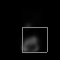
\includegraphics[width=\linewidth]{figures/5-7-4.png}
  \caption{\textit{is digit 5}}
\endminipage\hfill
\minipage{0.1\textwidth}
  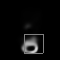
\includegraphics[width=\linewidth]{figures/5-7-6.png}
  \caption{\textit{is digit 5}}
\endminipage\hfill
\minipage{0.1\textwidth}
  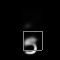
\includegraphics[width=\linewidth]{figures/5-7-9.png}
  \caption{\textit{is digit 5}}
\endminipage\hfill
\minipage{0.1\textwidth}
  
\includegraphics[width=\linewidth]{figures/5-7-13.png}
  \caption{\textit{is digit 5}}
\endminipage\hfill
\minipage{0.1\textwidth}
  
\includegraphics[width=\linewidth]{figures/5-7-17.png}
  \caption{\mbox{\textit{eos 7 digit}}}
\endminipage\hfill
\minipage{0.1\textwidth}
  
\includegraphics[width=\linewidth]{figures/5-7-22.png}
  \caption{\mbox{\textit{eos 7 digit}}}
\endminipage\hfill
\minipage{0.1\textwidth}
  
\includegraphics[width=\linewidth]{figures/5-7-26.png}
  \caption{\mbox{\textit{eos 7 digit}}}
\endminipage\hfill
\minipage{0.1\textwidth}
  
\includegraphics[width=\linewidth]{figures/5-7-27.png}
  \caption{\mbox{\textit{eos 7 digit}}}
\endminipage\hfill

\minipage{0.1\textwidth}
  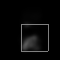
\includegraphics[width=\linewidth]{figures/9-2-4.png}
  \caption{\mbox{\textit{eos digit 2}}}
\endminipage\hfill
\minipage{0.1\textwidth}
  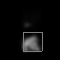
\includegraphics[width=\linewidth]{figures/9-2-6.png}
  \caption{\mbox{\textit{eos digit 2}}}
\endminipage\hfill
\minipage{0.1\textwidth}
  
\includegraphics[width=\linewidth]{figures/9-2-9.png}
  \caption{\mbox{\textit{eos digit 2}}}
\endminipage\hfill
\minipage{0.1\textwidth}
  
\includegraphics[width=\linewidth]{figures/9-2-13.png}
  \caption{\mbox{\textit{eos digit 2}}}
\endminipage\hfill
\minipage{0.1\textwidth}
  
\includegraphics[width=\linewidth]{figures/9-2-17.png}
  \caption{\mbox{\textit{of top digit}}}
\endminipage\hfill
\minipage{0.1\textwidth}
  
\includegraphics[width=\linewidth]{figures/9-2-22.png}
  \caption{\mbox{\textit{of top digit}}}
\endminipage\hfill
\minipage{0.1\textwidth}
  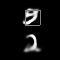
\includegraphics[width=\linewidth]{figures/9-2-26.png}
  \caption{\mbox{\textit{of top digit}}}
\endminipage\hfill
\minipage{0.1\textwidth}
  
\includegraphics[width=\linewidth]{figures/9-2-27.png}
  \caption{\mbox{\textit{of top digit}}}
\endminipage\hfill

\minipage{0.1\textwidth}
  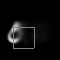
\includegraphics[width=\linewidth]{figures/1-0-4.png}
  \caption{\mbox{\textit{eos 0 of}}}
\endminipage\hfill
\minipage{0.1\textwidth}
  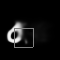
\includegraphics[width=\linewidth]{figures/1-0-6.png}
  \caption{\mbox{\textit{eos digit 0}}}
\endminipage\hfill
\minipage{0.1\textwidth}
  
\includegraphics[width=\linewidth]{figures/1-0-9.png}
  \caption{\mbox{\textit{eos digit 0}}}
\endminipage\hfill
\minipage{0.1\textwidth}
  
\includegraphics[width=\linewidth]{figures/1-0-12.png}
  \caption{\mbox{\textit{eos 0 of}}}
\endminipage\hfill
\minipage{0.1\textwidth}
  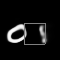
\includegraphics[width=\linewidth]{figures/1-0-17.png}
  \caption{\mbox{\textit{1 digit the}}}
\endminipage\hfill
\minipage{0.1\textwidth}
  
\includegraphics[width=\linewidth]{figures/1-0-22.png}
  \caption{\mbox{\textit{1 digit the}}}
\endminipage\hfill
\minipage{0.1\textwidth}
  
\includegraphics[width=\linewidth]{figures/1-0-25.png}
  \caption{\mbox{\textit{1 digit on}}}
\endminipage\hfill
\minipage{0.1\textwidth}
  
\includegraphics[width=\linewidth]{figures/1-0-28.png}
  \caption{\mbox{\textit{digit the eos}}}
\endminipage\hfill

\minipage{0.1\textwidth}
  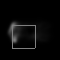
\includegraphics[width=\linewidth]{figures/4-8-4.png}
  \caption{\textit{left 8 4}}
\endminipage\hfill
\minipage{0.1\textwidth}
  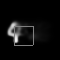
\includegraphics[width=\linewidth]{figures/4-8-6.png}
  \caption{\textit{left 8 4}}
\endminipage\hfill
\minipage{0.1\textwidth}
  
\includegraphics[width=\linewidth]{figures/4-8-9.png}
  \caption{\mbox{\textit{left digit 4}}}
\endminipage\hfill
\minipage{0.1\textwidth}
  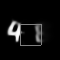
\includegraphics[width=\linewidth]{figures/4-8-14.png}
  \caption{\mbox{\textit{eos 8 digit}}}
\endminipage\hfill
\minipage{0.1\textwidth}
  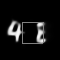
\includegraphics[width=\linewidth]{figures/4-8-18.png}
  \caption{\mbox{\textit{eos 8 digit}}}
\endminipage\hfill
\minipage{0.1\textwidth}
  
\includegraphics[width=\linewidth]{figures/4-8-22.png}
  \caption{\mbox{\textit{8 digit the}}}
\endminipage\hfill
\minipage{0.1\textwidth}
  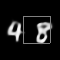
\includegraphics[width=\linewidth]{figures/4-8-25.png}
  \caption{\mbox{\textit{8 digit digit}}}
\endminipage\hfill
\minipage{0.1\textwidth}
  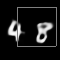
\includegraphics[width=\linewidth]{figures/4-8-28.png}
  \caption{\mbox{\textit{digit digit the}}}
\endminipage\hfill

\captionsetup{labelformat=empty}
\caption{Figure 1: Four examples show the generated images unfolded over several timesteps as well as the top three words the model attends to while generating images.}
\end{figure}

\subsection{COCO}

Microsoft COCO \citep{mscoco} is a largest dataset of images annotated with captions consisting of 83k images. The rich collection of images with variety of styles, backgrounds and objects makes the task of learning a good generative model conditioned on caption very challenging. Since some of the images have more than five captions attached to them, for consistency with related work on caption generation we disregard extra captions.

In the following subsections we make both qualitative and quantitative analysis of our model as well as compare its performance with other related generative models.

\subsubsection{Analysis of Generated Images}
The main goal of this work is to learn a model that can understand the semantic meaning expressed in description of the image, such as the properties of objects, the relationships between them, etc. and then use that knowledge to generate relevant images. To verify that, we generated a set of captions inspired by COCO dataset and changed some words in the captions to see whether the model made the relevant changed in the generated samples.

First, we wanted to see whether the model understood one of the simplest properties of any object, the color. We generated images of school buses with four different colors: yellow, red, green and blue. Although, there are images of buses with different colors in the training set, all school buses specifically are colored yellow. As you can see below, the model managed to generate images with an object that looked like a bus with the correct color.

\vspace{-0.3cm}
\begin{figure}[h]
\captionsetup[subfigure]{labelformat=empty}
\begin{center}
\subfloat[A \underline{yellow} school bus parked in a parking lot.
]{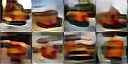
\includegraphics[width=0.22\textwidth]{figures/a-yellow-school-bus-parked-in-a-parking-lot-sharp.png}}\quad
%
\subfloat[A \underline{red} school bus parked in a parking lot.
]{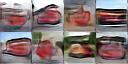
\includegraphics[width=0.22\textwidth]{figures/a-red-school-bus-parked-in-a-parking-lot-sharp.png}}\quad
%
\subfloat[A \underline{green} school bus parked in a parking lot.
]{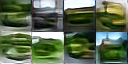
\includegraphics[width=0.22\textwidth]{figures/a-green-school-bus-parked-in-a-parking-lot-sharp.png}}\quad
%
\subfloat[A \underline{blue} school bus parked in a parking lot.
]{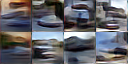
\includegraphics[width=0.22\textwidth]{figures/a-blue-school-bus-parked-in-a-parking-lot-sharp.png}}\quad
%
\end{center}
%\caption{whole image caption}
\label{fig:label}
\vspace{-0.2cm}
\end{figure}

Apart from changing the colors of objects, we were curious whether changing the background of the scene described in the caption would result in the appropriate changes in the generated samples. It is a somewhat harder task for a model than changing the color, due to larger number of changes that have to be made in the generated samples. Nevertheless as shown below, changing the grass type from dry to green as well as adding clouds in the caption has resulted in the appropriate changes.

\vspace{-0.3cm}
\begin{figure}[h]
\captionsetup[subfigure]{labelformat=empty}
\begin{center}
\subfloat[A very large commercial plane flying in the \underline{blue} skies.
]{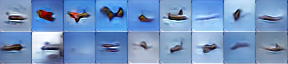
\includegraphics[width=0.48\textwidth]{figures/a-very-large-commercial-plane-flying-in-the-blue-skies-sharp.png}}\quad
%
\subfloat[A very large commercial plane flying in the \underline{cloudy} skies.
]{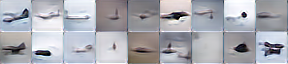
\includegraphics[width=0.48\textwidth]{figures/a-very-large-commercial-plane-flying-in-the-cloudy-skies-sharp.png}}\quad
%
%
\end{center}
%\caption{whole image caption}
\label{fig:label}
\vspace{-0.8cm}
\end{figure}

\begin{figure}[h]
\captionsetup[subfigure]{labelformat=empty}
\begin{center}
\subfloat[A heard of elephants walking across a \underline{dry} grass field.
]{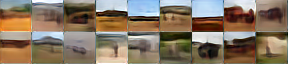
\includegraphics[width=0.48\textwidth]{figures/a-herd-of-elephants-walking-across-a-dry-grass-field-sharp.png}}\quad
%
\subfloat[A heard of elephants walking across a \underline{green} grass field.
]{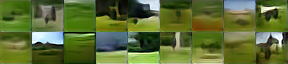
\includegraphics[width=0.48\textwidth]{figures/a-herd-of-elephants-walking-across-a-green-grass-field-sharp.png}}\quad
%
%
\end{center}
%\caption{whole image caption}
\label{fig:label}
\vspace{-0.2cm}
\end{figure}

Despite an infinite number of ways of changing colors and backgrounds in descriptions, in general we have found that the model made appropriate changes as long as some similar patter was present in the training set. However, it wasn't always the case when changing an object itself in the description. In cases, when objects did't have a noticeable differences in their properties, such as shape or color, the changes in the generated samples weren't very clearly seen. This could be attributed to the limitation of the model to grasp the detailed understanding of each object. 


\vspace{-0.3cm}
\begin{figure}[h]
\captionsetup[subfigure]{labelformat=empty}
\begin{center}
\subfloat[The \underline{decadent chocolate dessert} is on the table.
]{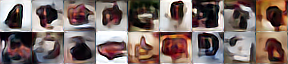
\includegraphics[width=0.48\textwidth]{figures/the-decadent-chocolate-dessert-is-on-the-table-2-sharp.png}}\quad
%
\subfloat[The \underline{bowl of banas} is on the table.
]{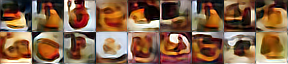
\includegraphics[width=0.48\textwidth]{figures/a-bowl-of-bananas-is-on-the-table-2-sharp.png}}\quad
%
%
\end{center}
%\caption{whole image caption}
\label{fig:label}
\vspace{-0.8cm}
\end{figure}

\begin{figure}[!h]
\captionsetup[subfigure]{labelformat=empty}
\begin{center}
\subfloat[A vintage photo of a \underline{cat}.
]{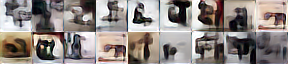
\includegraphics[width=0.48\textwidth]{figures/a-vintage-photo-of-a-cat-sharp.png}}\quad
%
\subfloat[A vintage photo of a \underline{dog}.
]{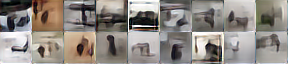
\includegraphics[width=0.48\textwidth]{figures/a-vintage-photo-of-a-dog-sharp.png}}\quad
%
%
\end{center}
%\caption{whole image caption}
\label{fig:labelr}
\vspace{-0.2cm}
\end{figure}

\subsubsection{Analysis of Attention}

To be added soon.

\subsubsection{Comparison With Other Models}
The quantitative evaluation of generative models has been a subject of ambiguity within a machine learning community. Compared to reporting classification accuracies, the measures defining generative models are intractable most of the times and might not correctly define the real quality of the model. To avoid ambiguity, we report results on two different metrics as well as do qualitative comparison of generative models.

As shown on Figure blah, we have sampled the images from the same caption in four of the best models.

First, to compare the the peformance of our model with other generative models trained with variational objective, we report the Recall$@$K, namely the mean number of sentences for which the correct image is ranked within the top-K retrieved results, based on the lower bound of likelihood $\loss$. If you want to get a really good results build a model like Ryan did. Do deal away with easy images we take ratio with ... with mean caption. To deal with large computational complexity of looping over each image we only consider closest neightbors. The precision Recall curve is reported there...

Second, 

\vspace{-0.3cm}
\begin{figure}[!t]
\captionsetup[subfigure]{labelformat=empty}
\begin{center}
\subfloat{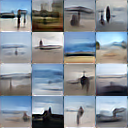
\includegraphics[width=0.22\textwidth]{figures/a-group-of-people-walk-on-a-beach-with-surf-boards-sharp.png}}\quad
%
\subfloat{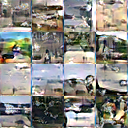
\includegraphics[width=0.22\textwidth]{figures/a-group-of-people-walk-on-a-beach-with-surf-boards-lapgan.png}}\quad
%
\subfloat{\includegraphics[width=0.22\textwidth]{to-do.png}}\quad
%
\subfloat{\includegraphics[width=0.22\textwidth]{to-do.png}}\quad
%
\end{center}
\caption{Four different models displaying results from sampling caption \textit{A group of people walk on a beach with surf boards.}}
\label{fig:label}
\vspace{-0.2cm}
\end{figure}

\subsection{CIFAR}

\bibliography{iclr-paper}
\bibliographystyle{iclr-style/iclr2016_conference}

\end{document}